\documentclass[tikz,border=1pt]{standalone}
\usepackage[T1]{fontenc}
\usepackage[utf8]{inputenc}
\usepackage[english]{babel}
\usepackage{array,amsmath,amssymb,mathtools,microtype,tikz}
\usetikzlibrary{shapes.geometric,patterns,positioning}

\usepackage{pgfplots}
\pgfplotsset{compat=1.13}
\usetikzlibrary{backgrounds,calc,decorations.pathreplacing}
\usepgfplotslibrary{groupplots}

% IEEE
%\renewcommand{\sfdefault}{phv}
%\renewcommand{\rmdefault}{ppl}
%\renewcommand{\ttdefault}{pcr}
%\usepackage{mathptmx}

% ACM
\usepackage[tt=false, type1=true]{libertine}
\usepackage[varqu]{zi4}
\usepackage[libertine]{newtxmath}

\usetikzlibrary{arrows.meta,calc,shapes.arrows,decorations.pathreplacing,shadows,backgrounds}
\usepackage{pgfplots}
\pgfplotsset{compat=1.16}
\usepgfplotslibrary{groupplots}
\usepgfplotslibrary{colormaps}
\tikzset{
	bar-color/.style={
		color of colormap={#1},
		draw=.!80!black,
		fill=.!80!white,
	},
	normal-color/.style={
		color of colormap={#1},
		draw=.,
	},
	mark-color/.style={
		color of colormap={#1},
		draw=.!80!black,
		fill=.!80!white,
	},
	mydashed/.style={dash pattern=on 6pt off 4pt}
}


\begin{document}
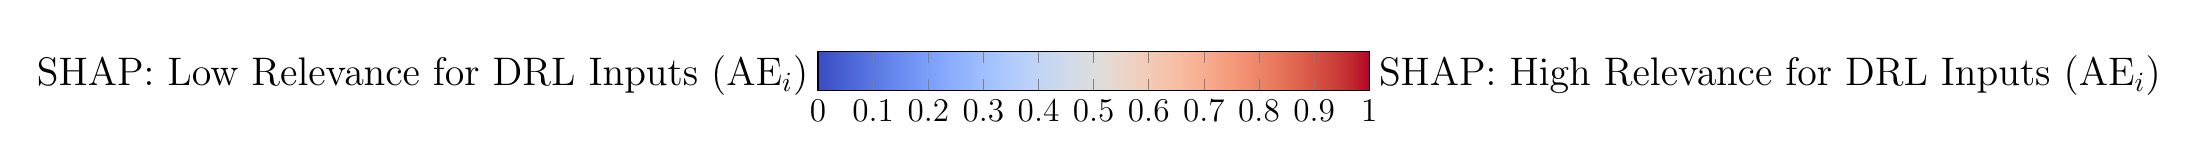
\begin{tikzpicture}[text depth=0pt]
\begin{axis}[
	hide axis,
	scale only axis,
	height=0pt,
	width=0pt,
	colormap={mymap}{[1pt]
		rgb(0pt)=(0.2298057,0.298717966,0.753683153);
		rgb(1pt)=(0.26623388,0.353094838,0.801466763);
		rgb(2pt)=(0.30386891,0.406535296,0.84495867);
		rgb(3pt)=(0.342804478,0.458757618,0.883725899);
		rgb(4pt)=(0.38301334,0.50941904,0.917387822);
		rgb(5pt)=(0.424369608,0.558148092,0.945619588);
		rgb(6pt)=(0.46666708,0.604562568,0.968154911);
		rgb(7pt)=(0.509635204,0.648280772,0.98478814);
		rgb(8pt)=(0.552953156,0.688929332,0.995375608);
		rgb(9pt)=(0.596262162,0.726149107,0.999836203);
		rgb(10pt)=(0.639176211,0.759599947,0.998151185);
		rgb(11pt)=(0.681291281,0.788964712,0.990363227);
		rgb(12pt)=(0.722193294,0.813952739,0.976574709);
		rgb(13pt)=(0.761464949,0.834302879,0.956945269);
		rgb(14pt)=(0.798691636,0.849786142,0.931688648);
		rgb(15pt)=(0.833466556,0.860207984,0.901068838);
		rgb(16pt)=(0.865395197,0.86541021,0.865395561);
		rgb(17pt)=(0.897787179,0.848937047,0.820880546);
		rgb(18pt)=(0.924127593,0.827384882,0.774508472);
		rgb(19pt)=(0.944468518,0.800927443,0.726736146);
		rgb(20pt)=(0.958852946,0.769767752,0.678007945);
		rgb(21pt)=(0.96732803,0.734132809,0.628751763);
		rgb(22pt)=(0.969954137,0.694266682,0.579375448);
		rgb(23pt)=(0.966811177,0.650421156,0.530263762);
		rgb(24pt)=(0.958003065,0.602842431,0.481775914);
		rgb(25pt)=(0.943660866,0.551750968,0.434243684);
		rgb(26pt)=(0.923944917,0.49730856,0.387970225);
		rgb(27pt)=(0.89904617,0.439559467,0.343229596);
		rgb(28pt)=(0.869186849,0.378313092,0.300267182);
		rgb(29pt)=(0.834620542,0.312874446,0.259301199);
		rgb(30pt)=(0.795631745,0.24128379,0.220525627);
		rgb(31pt)=(0.752534934,0.157246067,0.184115123);
		rgb(32pt)=(0.705673158,0.01555616,0.150232812);
	},
	colorbar horizontal,
	point meta min=0,
	point meta max=1,
	colorbar style={
		width=7cm,
		xtick={0,0.1,...,1},
		xticklabel style={font=\large}
	}]
	\addplot [draw=none] coordinates {(0,0)};
\end{axis}
\node [anchor=west,font=\Large] at (7,-0.55)  {SHAP: High Relevance for DRL Inputs (AE$_i$)};
\node [anchor=east,font=\Large] at (0,-0.55)  {SHAP: Low Relevance for DRL Inputs (AE$_i$)};
\end{tikzpicture}
\end{document}